\documentclass[9pt,twocolumn,twoside,]{pnas-new}

% Use the lineno option to display guide line numbers if required.
% Note that the use of elements such as single-column equations
% may affect the guide line number alignment.


\usepackage[T1]{fontenc}
\usepackage[utf8]{inputenc}

% tightlist command for lists without linebreak
\providecommand{\tightlist}{%
  \setlength{\itemsep}{0pt}\setlength{\parskip}{0pt}}


% Pandoc citation processing
\newlength{\cslhangindent}
\setlength{\cslhangindent}{1.5em}
\newlength{\csllabelwidth}
\setlength{\csllabelwidth}{3em}
\newlength{\cslentryspacingunit} % times entry-spacing
\setlength{\cslentryspacingunit}{\parskip}
% for Pandoc 2.8 to 2.10.1
\newenvironment{cslreferences}%
  {}%
  {\par}
% For Pandoc 2.11+
\newenvironment{CSLReferences}[2] % #1 hanging-ident, #2 entry spacing
 {% don't indent paragraphs
  \setlength{\parindent}{0pt}
  % turn on hanging indent if param 1 is 1
  \ifodd #1
  \let\oldpar\par
  \def\par{\hangindent=\cslhangindent\oldpar}
  \fi
  % set entry spacing
  \setlength{\parskip}{#2\cslentryspacingunit}
 }%
 {}
\usepackage{calc}
\newcommand{\CSLBlock}[1]{#1\hfill\break}
\newcommand{\CSLLeftMargin}[1]{\parbox[t]{\csllabelwidth}{#1}}
\newcommand{\CSLRightInline}[1]{\parbox[t]{\linewidth - \csllabelwidth}{#1}\break}
\newcommand{\CSLIndent}[1]{\hspace{\cslhangindent}#1}


\templatetype{pnasresearcharticle}  % Choose template

\title{Oiseaux ou pas oiseaux, telle est la question!}

\author[]{Thomas Cournoyer}
\author[]{Félix Richard}
\author[]{Liam Ryan}
\author[]{Xavier Delisle}

  \affil[]{Université de Sherbrooke, Cour BIO500}


% Please give the surname of the lead author for the running footer
\leadauthor{}

% Please add here a significance statement to explain the relevance of your work
\significancestatement{}


\authorcontributions{}



\correspondingauthor{\textsuperscript{} }

% Keywords are not mandatory, but authors are strongly encouraged to provide them. If provided, please include two to five keywords, separated by the pipe symbol, e.g:


\begin{abstract}
Résumé
\end{abstract}

\dates{This manuscript was compiled on \today}
\doi{\url{www.pnas.org/cgi/doi/10.1073/pnas.XXXXXXXXXX}}

\begin{document}

% Optional adjustment to line up main text (after abstract) of first page with line numbers, when using both lineno and twocolumn options.
% You should only change this length when you've finalised the article contents.
\verticaladjustment{-2pt}



\maketitle
\thispagestyle{firststyle}
\ifthenelse{\boolean{shortarticle}}{\ifthenelse{\boolean{singlecolumn}}{\abscontentformatted}{\abscontent}}{}

% If your first paragraph (i.e. with the \dropcap) contains a list environment (quote, quotation, theorem, definition, enumerate, itemize...), the line after the list may have some extra indentation. If this is the case, add \parshape=0 to the end of the list environment.

\acknow{}

\hypertarget{introduction}{%
\section*{Introduction}\label{introduction}}
\addcontentsline{toc}{section}{Introduction}

Définition et explication de la ou les question du projet Observer
l'influence que la géographie et la période temporelle ont sur la
diversité d'espèce dans la répartition des données du québec

\hypertarget{muxe9thodes-et-ruxe9sultats}{%
\section*{Méthodes et résultats}\label{muxe9thodes-et-ruxe9sultats}}
\addcontentsline{toc}{section}{Méthodes et résultats}

Une courte description de la méthode et des résultats

\hypertarget{submitting-manuscripts}{%
\section*{Discussion}\label{submitting-manuscripts}}
\addcontentsline{toc}{section}{Discussion}

Une discussion, enrichie de citations provenant de la littérature
scientifique

\hypertarget{references}{%
\subsection*{References}\label{references}}
\addcontentsline{toc}{subsection}{References}

References should be cited in numerical order as they appear in text;
this will be done automatically via bibtex, e.g. (1) and (2, 3). All
references, including for the SI, should be included in the main
manuscript file. References appearing in both sections should not be
duplicated. SI references included in tables should be included with the
main reference section.

\begin{figure}
\centering
\includegraphics[width=0.1\textwidth,height=0.1\textheight]{"../Rapport/frog.png"}
\caption{Légende figure. \label{fig:plot1}}
\end{figure}

\hypertarget{sec:figures}{%
\subsection*{Digital Figures}\label{sec:figures}}
\addcontentsline{toc}{subsection}{Digital Figures}

\begin{figure}
\centering
\includegraphics{frog.png}
\caption{Placeholder image of a frog with a long example caption to show
justification setting.{}}
\end{figure}

\hypertarget{sec:figures}{%
\subsection*{Digital Figures}\label{sec:figures}}
\addcontentsline{toc}{subsection}{Digital Figures}

\begin{figure}
\centering
\includegraphics{frog.png}
\caption{Placeholder image of a frog with a long example caption to show
justification setting.{}}
\end{figure}

\hypertarget{sec:figures}{%
\subsection*{Digital Figures}\label{sec:figures}}
\addcontentsline{toc}{subsection}{Digital Figures}

Figures and Tables should be labelled and referenced in the standard way
using the \texttt{\textbackslash{}label\{\}} and
\texttt{\textbackslash{}ref\{\}} commands.

Figure \[fig:frog\] shows an example of how to insert a column-wide
figure. To insert a figure wider than one column, please use the
\texttt{\textbackslash{}begin\{figure*\}...\textbackslash{}end\{figure*\}}
environment. Figures wider than one column should be sized to 11.4 cm or
17.8 cm wide.

\hypertarget{single-column-equations}{%
\subsection*{Single column equations}\label{single-column-equations}}
\addcontentsline{toc}{subsection}{Single column equations}

Authors may use 1- or 2-column equations in their article, according to
their preference.

To allow an equation to span both columns, options are to use the
\texttt{\textbackslash{}begin\{figure*\}...\textbackslash{}end\{figure*\}}
environment mentioned above for figures, or to use the
\texttt{\textbackslash{}begin\{widetext\}...\textbackslash{}end\{widetext\}}
environment as shown in equation \[eqn:example\] below.

Please note that this option may run into problems with floats and
footnotes, as mentioned in the \href{http://texdoc.net/pkg/cuted}{cuted
package documentation}. In the case of problems with footnotes, it may
be possible to correct the situation using commands
\texttt{\textbackslash{}footnotemark} and
\texttt{\textbackslash{}footnotetext}.

\[\begin{aligned}
(x+y)^3&=(x+y)(x+y)^2\\
       &=(x+y)(x^2+2xy+y^2) \label{eqn:example} \\
       &=x^3+3x^2y+3xy^3+x^3. 
\end{aligned}\]

\showmatmethods

\hypertarget{references}{%
\section*{Références}\label{references}}
\addcontentsline{toc}{section}{Références}

\pnasbreak

\hypertarget{refs}{}
\begin{CSLReferences}{0}{0}
\leavevmode\vadjust pre{\hypertarget{ref-belkin2002using}{}}%
\CSLLeftMargin{1. }%
\CSLRightInline{Belkin M, Niyogi P (2002) Using manifold stucture for
partially labeled classification. \emph{Advances in Neural Information
Processing Systems}, pp 929--936.}

\leavevmode\vadjust pre{\hypertarget{ref-berard1994embedding}{}}%
\CSLLeftMargin{2. }%
\CSLRightInline{Bérard P, Besson G, Gallot S (1994) Embedding riemannian
manifolds by their heat kernel. \emph{Geometric \& Functional Analysis
GAFA} 4(4):373--398.}

\leavevmode\vadjust pre{\hypertarget{ref-coifman2005geometric}{}}%
\CSLLeftMargin{3. }%
\CSLRightInline{Coifman RR, et al. (2005) Geometric diffusions as a tool
for harmonic analysis and structure definition of data: Diffusion maps.
\emph{Proceedings of the National Academy of Sciences of the United
States of America} 102(21):7426--7431.}

\end{CSLReferences}



% Bibliography
% \bibliography{pnas-sample}

\end{document}
